
\begin{frame}[fragile]{Kokkos User Group Meeting 2025}
\begin{center}
\textbf{What to expect from KUG}
\end{center}

\begin{center}
  Eight 90-minute sessions featuring a dynamic blend of Kokkos developers and community users
\end{center}

  \begin{multicols}{2}
    \textit{Day 1 Sessions:}
      \begin{itemize}
        \item{09:00-10:20 \textbf{Essential Updates}}
        \item{10:45-12:05 \textbf{Kokkos in Applications}}
        \item{01:35-03:15 \textbf{Adopting Kokkos}}
        \item{03:40-\textcolor{red}{05:10} \textbf{Lightning Talks}}
    \end{itemize}

    \columnbreak

    \textit{Day 2 Sessions:}
      \begin{itemize}
        \item{09:00-10:20 \textbf{Kokkos Ecosystem}}
        \item{10:45-12:05 \textbf{Tuning and Perf.}}
        \item{01:35-03:15 \textbf{Algorithms}}
        \item{03:40-05:00 \textbf{Panel Discussion}}
    \end{itemize}
  \end{multicols}
\end{frame}

\begin{frame}[fragile]{Audience @ KUG}
\begin{center}
\textbf{Diverse audience @ KUG 2025}
\vspace{0.5cm}

  \begin{itemize}
    \item{\textbf{DOE Laboratories}: SNL,ORNL,LANL,ANL,LLNL}
    \item{\textbf{Non-DOE}:CEA,CIRA,C-DAC,CSCS MPI,CINES,FZJ, Stoney Brook, UT Austin, University of Oregon, Princeton University, University de Liege, Tennessee Technical University}
    \item{\textbf{Number of Talks}: 33 with 14 DOE affiliation, 19 other}
    \item{\textbf{Nationalities}: US, France, Germany, India, Switzerland, Belgium}
  \end{itemize}

\end{center}
\end{frame}

\begin{frame}[fragile]{When to look pretty}
\begin{center}
\textbf{We would like to take a group picture today at 12:05, the start of the lunch break}
\vspace{0.5cm}
\end{center}
\end{frame}


\begin{frame}[fragile]{Release timeline}
\begin{center}
\textbf{We try to release on a 4 month cycle}
\vspace{1cm}

    \begin{tikzpicture}
\begin{axis}[
    width=\textwidth,
    date coordinates in=x,
    % date ZERO=2023-03-03,
    date ZERO=2020-01-31,
    % xmin=2023-01-03 00:00, xmax=2026-03-20 00:00,
    xmin=2019-11-03 00:00, xmax=2026-03-20 00:00,
    xtick={2019-11-03,2020-03-03,2020-07-03,2020-11-03,2021-03-03,2021-07-03,2021-11-03,2022-03-03,2022-07-03,2022-11-03,2023-03-03,2023-07-03,2023-11-03,2024-03-03,2024-07-03,2024-11-03,2025-03-03,2025-07-03,2025-11-03,2026-03-03},
    axis x line=bottom,% only show the bottom x axis
    xticklabel style={rotate=90,anchor=near xticklabel},
    xticklabel={\pgfcalendarmonthshortname{\month}/\year},
    hide y axis,
    ymin=0,ymax=6,
    y=0.2cm,
    scatter/classes={%
        a={mark=o,draw=black}}
    ]

\addplot[scatter,only marks,mark=x,
    mark size = 3pt,
    color = green]
coordinates {
  (2020-01-31 00:00, 1)
  (2020-04-14 00:00, 1)
  (2020-08-19 00:00, 1)
  (2020-12-16 00:00, 1)
  (2021-04-26 00:00, 1)
  (2021-11-19 00:00, 1)
  (2022-04-14 00:00, 1)
  (2022-08-25 00:00, 1)
    };
    \node [coordinate,pin=above:{3.0}]
        at (axis cs:2020-01-31,1)   {};
    \node [coordinate,pin=above:{3.7}]
        at (axis cs:2022-08-25,1) {};

\addplot[scatter,only marks,mark=x,
    mark size = 3pt,
    color = red]
coordinates {
  (2023-03-03 00:00, 1)
  (2023-06-28 00:00, 1)
  (2023-11-20 00:00, 1)
  (2024-04-04 00:00, 1)
  (2024-08-12 00:00, 1)
  (2024-11-25 00:00, 1)
  (2025-03-28 00:00, 1)
    };
    \node [coordinate,pin=above:{4.0}]
        at (axis cs:2023-03-03,1)   {};
    \node [coordinate,pin=above:{4.6}]
        at (axis cs:2025-03-28,1) {};

\addplot[scatter,only marks,mark=x,
    mark size = 3pt,
    color = black!40!white]
coordinates {
  (2025-07-20 00:00, 1)
  (2025-11-20 00:00, 1)
    };

    \node [coordinate,pin=above:{4.7}]
        at (axis cs:2025-07-20,1)   {};
    \node [coordinate,pin=above:{5.0}]
        at (axis cs:2025-11-20,1) {};

\end{axis}
\end{tikzpicture}
\end{center}

\end{frame}

\begin{frame}[fragile]{Upcoming Releases}
  \begin{center}
\textbf{Kokkos 5.0 is coming soon!}
\vspace{1cm}
  \begin{itemize}
    \item{\textbf{4.6}: 03/2025}
    \item{\textbf{4.7}: \textcolor{black!40!white}{07/2025}}
    \item{\textbf{5.0}: \textcolor{black!40!white}{11/2025} Will require c++ 20!}
  \end{itemize}
  \end{center}
\end{frame}

\begin{frame}[fragile]{Thanks to all the speakers}

  \begin{center}
  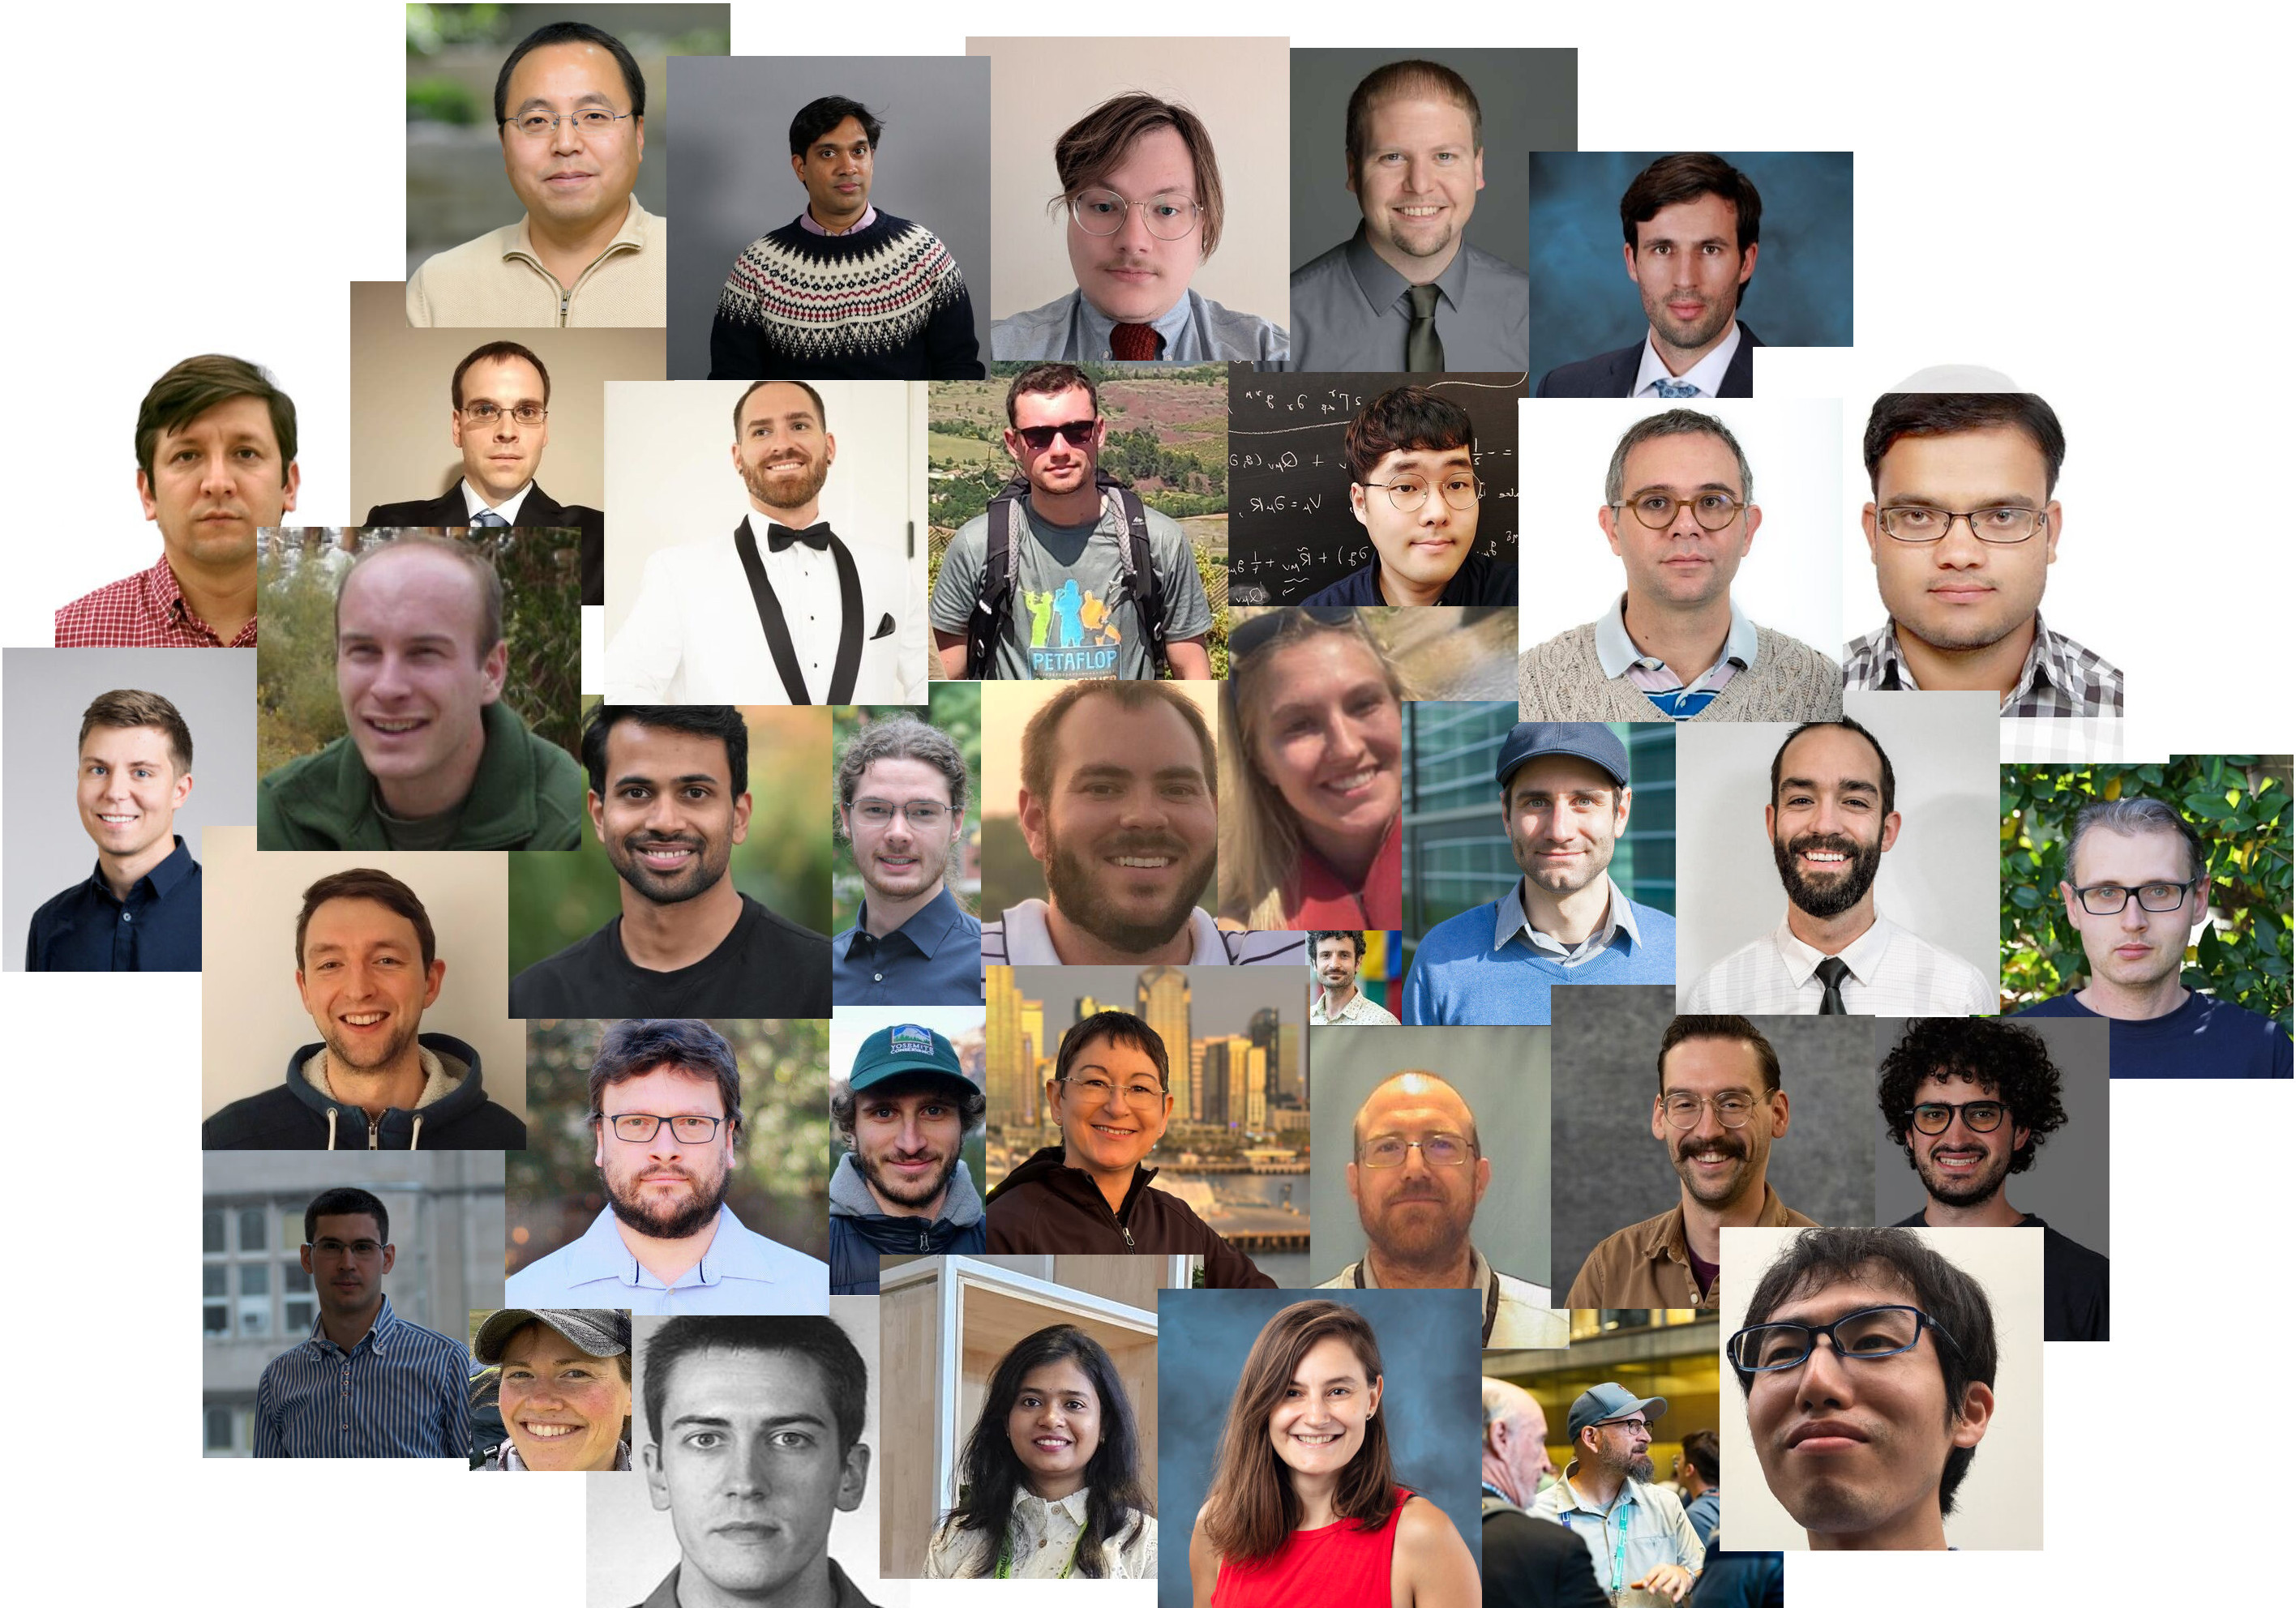
\includegraphics[height=0.8\textheight]{mosaic.jpg}
  \end{center}

\end{frame}
